\documentclass[a4paper]{article}
\usepackage[utf8]{inputenc}
\usepackage[natbib,sorting=none]{biblatex}
\usepackage{graphicx}
\usepackage{acronym}
\usepackage{indentfirst}
\usepackage[none]{hyphenat}
\usepackage{fancyhdr}
\usepackage{enumitem}
\usepackage{listings}
\usepackage{xcolor}
\usepackage{pifont}

\addbibresource{references.bib}
\newcommand{\comment}[1]{\textbf{[Comment: #1]}}

\begin{document}
\setlist[enumerate]{label=\alph*),leftmargin=0.4cm, topsep=0cm}
\setlist[itemize]{leftmargin=0.4cm, topsep=0cm}
\begin{figure}[!h]
	\centering
	
\includegraphics[width=80mm]{images/poli-logo.png}
\end{figure}
\hfill
\begin{center}
    \fontsize{18px}{6mm}\selectfont \textsc{\textbf{Software Engineering II project}}
\end{center}
\begin{center}
    \fontsize{12px}{4mm}\selectfont \textsc{Academic Year: 2018/2019}
\end{center}
\hfill
\hfill
\begin{figure}[!h]
	\centering
	
\includegraphics[width=120mm]{images/trackme-logo.png}
\end{figure}
\hfill
\hfill
\begin{center}
    \fontsize{22px}{8mm}\selectfont \textsc{\textbf{Requirement Analysis and\\ Specification Document}}
\end{center}
\begin{center}
    \fontsize{14px}{4mm}\selectfont \textsc{{Draft Version 0.1 - 11/10/2018}}
\end{center}
\hfill
\hfill
\begin{center}
\fontsize{14px}{4mm}\selectfont \textsc{\textit{Davide Rutigliano -  903616}}
\end{center}

\begin{center}
\fontsize{14px}{4mm}\selectfont \textsc{\textit{Claudio Ferrante - 903417\\}}
\end{center}

\begin{center}
\fontsize{14px}{4mm}\selectfont \textsc{\textit{Davide Matta - 903616}}
\end{center}
\pagenumbering{roman}
\tableofcontents
\rfoot{
\includegraphics[width=30mm]{Images/trackme-logo-mini.png}}

%%%%%%%%%%%%%%%%%%%%%%%%%%%%%%%%%%%%%%%%%%%%%%%%%%%%%%%%%%%%%%%%%%%%%%
\newpage
\pagestyle{fancy}
\pagenumbering{arabic}

\section{Introduction}
\subsection{Purpose}
    The Purpose of this Design Document is to provide, in a more specific and technical way with respect to the RASD, all the details of \textit{TrackMe} system \cite{rasd}. The \textit{Requirement Analysis and Specification Document} is also recommended to developer aimed at implementing the proposed system.
    
    The purpose of this paper is to point out the main components, their interfaces and their behaviours, show the high level architecture and its interaction with architectural components and to identify style and design patterns that shall be used in deployment of the application. This Document will provide detailed explanation of each functionality through components and sequence diagrams also used to explain to programmers the overall structure of the system in a precise and implementation-oriented way.
    
    Furthermore this document provides also an \textit{Implementation \& Test} plan in order to give to the developer a precise idea of the deployment process.
 
\subsection{Scope}
    \textit{TrackMe} allows Third-Party to access Individual's health data exploiting the functionality of \textit{Data4help} service: Third-Parties can make individual requests that the Individuals can accept or reject, or group requests handled directly by TrackMe that approves them if it is able to properly anonymize the requested data. For sake of simplicity, we already assumed that TrackMe will accept any request for which the number of individuals whose data satisfy the request is higher than 1000. The application may also allow individual users to connect external devices such as smart-watches, specific pathology's monitoring devices or other types of external devices able to monitor health parameters with BT or NFC connection.

    In addition, the system permits to enable the \textit{Automated-SOS} service that guarantees that the GPS position of the user who has enabled \textit{Automated SOS}, can be send to the nearest ambulance available, when user's health parameters overcome some critical thresholds. This procedure takes place thanks to an ambulance dispatcher, which is connected to the Third-Party (which has enabled automated-SOS too), that has been selected by that individual to provide this service
   
    Moreover, through  the \textit{Track4Run} service, \textit{TrackMe} allows \textit{Organizers} (that are individuals)  to  \textit{create}  a  new  run:  a  competition  in  which other individuals can either participate as \textit{athletes} or watch as \textit{spectators}.  Additionally, this feature guarantees other services for keeping track of athletes progresses during the run, providing an interactive map of the run, with runners position on it.
    
\subsection{Definition, Acronyms and  Abbreviations}
            \subsubsection{Keywords}
            The key words “MUST”, “MUST NOT”, “REQUIRED”, “SHALL”, “SHALL NOT”, “SHOULD”, “SHOULD NOT”, “RECOMMENDED”, “MAY”, and “OPTIONAL” in this document are to be interpreted as described in RFC 2119 \cite{bradner1997key}.
            
            \subsubsection{Definition of Terms}
            This document uses several terms that might be more loosely used elsewhere. These terms are defined here as they will be used later on in this document.
                \begin{description}
                    \item[\textbf{Subscribed User}] an Individual for which one Third Party whom asked to subscribe to the data has accepted the Third Party's request
                    
                    \item[\textbf{External Device}] a device such as a smart-watch or similar, capable of data acquisition
                    
                    \item[\textbf{Run}] a competition organized and managed by an \textit{Organizer} to which \textit{Athletes} and \textit{Spectators} can enroll as participant or watchers
                    
                    \item[\textbf{Run Started}] a competition with at least two \textit{Athletes} enrolled that the \textit{Organizer} has started
                    
                    \item[\textbf{Run Created}] a competition with any number of \textit{Athletes} enrolled
                    
                    \item[\textbf{Track}] A route where athletes will compete in a specific \textit{Run}
                    
                    \item[\textbf{Map}] A \textit{Track} that display all \textit{Athletes} position in a specific \textit{Run}
                    
                    \item[Accident] An event triggered when the monitored user's parameter overcome certain thresholds
                    
                    \item[\textbf{TrackMe}] the \textit{"system to be"}
                    
                    \item[\textbf{Data4Help}] a data monitoring service provided by \textit{TrackMe}
                    
                    \item[\textbf{Automated-SOS}] an SOS service built on top of \textit{Data4Help}
                    
                    \item[\textbf{Track4Run}] run management service offered by \textit{TrackMe} application
                    
                    \item[\textbf{Credential}] as used in this document, is a combination of both username and password used by an \textit{User} to authenticate him/herself during the Log-in phase
                    
                    \item[\textbf{Personal Data}] users' data of different kind either for Individuals (name, surname, age, etc.) or for Third-Parties such as Organization name, number of employees or VAT number
                \end{description}
            
            \subsubsection{Acronyms}
            \begin{acronym}
                \acro{DD}{Design Document}
                \acro{UML}{Unified Modelling Language}
                \acro{SQL}{Structured Query Language}
                \acro{noSQL}{Not Only SQL}
                \acro{REST}{REpresentational State Transfer}
                \acro{API}{Application Programming Interface}
                \acro{RASD}{Requirement Analysis and Specification Document}
                \acro{UX}{User eXperience}
            \end{acronym}
            
\subsection{Reference Documents}
\printbibliography[heading=none]

%%%%%%%%%%%%%%%%%%%%%%%%%%%%%%%%%%%%%%%%%%%%%%%

\subsection{Document Structure}
\begin{itemize}
    \item \textbf{Introduction}: this section is aimed at giving to the reader an overview of the document;

\item \textbf{Architecture Design}:
\begin{enumerate}
    \item \textit{High Level Components and their Interaction}: gives a global view of the components of the application and how they communicate;

    \item \textit{Component View}: gives a more detailed view of the components of the applications through UML component diagrams;

    \item \textit{Deployment View}: shows UML deployment diagrams and their explanations;
    
    \item \textit{Entity Relation Diagram}: shows database entities and relationships;

    \item \textit{Runtime View}: presents UML sequence diagrams in order to show the event flow of the different tasks of the application;

    \item \textit{Component Interfaces}: presents the interfaces between the components;

    \item \textit{Selected Architectural Styles and Patterns}: explain the architectural choices done during the design of the application and design patterns;

    \item \textit{Other design decisions};
\end{enumerate}

\item \textbf{Algorithms Design}: this chapter describes the most critical parts via some algorithms. Pseudo code is used in order to hide unnecessary implementation details and in order to focus on the most important parts;

\item \textbf{User Interface Design}: this part presents mockups and user experience explained via mockups and UX diagrams;

\item \textbf{Requirements Traceability}: this section aims to explain how the decisions taken in the RASD are linked to design elements in the Design Document.
\end{itemize}

\newpage
\section{Architectural Design}
\subsection{High Level Components and their Interaction}
The system is deployed on three different tiers: the data layer, the application layer and the presentation layer, that are respectively mapped on the three main components of the software application.
\begin{figure}[!htpb]
    	\centering
    	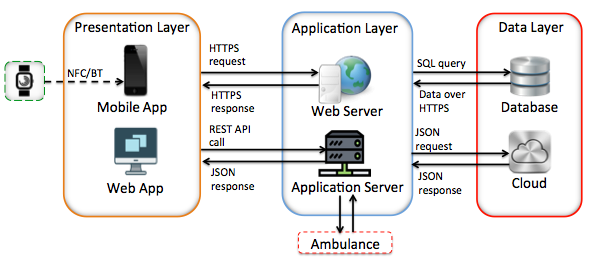
\includegraphics[width=100mm,keepaspectratio]{images/highlevel.png}
    	\caption{High Level interaction diagram}
\end{figure}

The main component is the system itself and includes both the \textit{Web Server} and the \textit{Application Server}. The former communicates in synchronous way over HTTPS with client browser or mobile application, while the latter manages all the application logic and it is interfaced with the \textit{Data Layer}. Furthermore, the \textit{Presentation Layer} can also \textit{consume} REST services made available by the \textit{Application Server}. The \textit{Data Layer} instead is composed of two sub-components: a classic SQL database or optionally a less traditional noSQL database (e.g. MongoDB).

Moreover, both the \textit{Application Layer} and the \textit{Presentation Layer} should interact with external services:
\begin{itemize}
    \item The \textit{Mobile Application} may be connected with an external device such as smart-watches, specific pathology's monitoring devices or other types of external devices able to monitor health parameters with BT or NFC connection;
    \item The \textit{Application Server} should be able to communicate with ambulances in order to send them individual's position and notify them in case of accident.
\end{itemize}

\begin{figure}[!htpb]
    	\centering
    	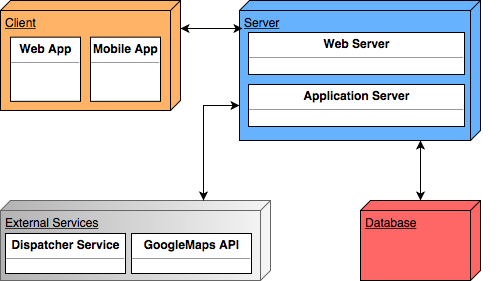
\includegraphics[width=100mm,keepaspectratio]{images/highlevel2.png}
    	\caption{High Level components diagram}
\end{figure}

\subsection{Component View}
\newpage
\subsection{Deployment View}
\comment{fix this plzzz}
\begin{figure}
    \centering
    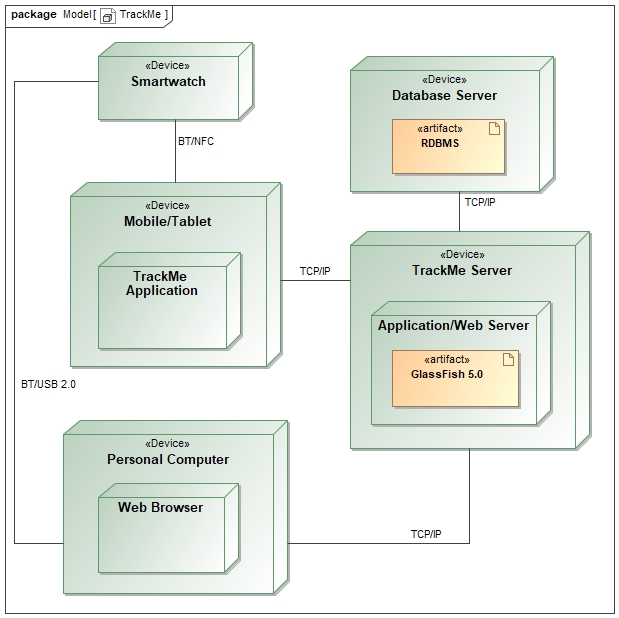
\includegraphics[width=\textwidth,keepaspectratio]{images/UML/deployment_TrackMe.jpg}
    \caption{TrackMe Deployment Diagram}
    \label{fig:deployment_trackme}
\end{figure}


\subsection{Entity Relation Diagram}

\subsection{Runtime View}

\subsection{Component Interfaces}

\subsection{Selected Architectural Styles and Patterns}
    \subsubsection{Architecture Style}
    \subsubsection{Design Patterns}
    \subsubsection{RESTful API}
    \begin{table}[!htpb]
        \begin{tabular}{|p{3cm}|p{1.8cm}|p{1.8cm}|p{1.8cm}|p{1.8cm}|} 
         \hline
         \textbf{Resource} & \textbf{GET} & \textbf{POST} & \textbf{PUT} & \textbf{DELETE} \\
         \hline
         \textit{trackMe/individual} & sth &like & this & ? \\
         \hline
        \end{tabular}
    \end{table}

\subsection{Other Design Decisions}

\newpage
\section{User Interface Design}
As specified in RASD there are two different user interfaces, one for mobile application and one for web browsers. In this specification we assume the web version of the application will be the same as the mobile application with reduced functions.

\subsection{Mockups}
The guest who access to the main page can sign-up to the application providing his credentials. Once clicked on the \textit{Sign On} button the guest can decide whether registers as an Individual or as a Third-Party, swiping left and right to choose the wright option. Once registered, on initial page, an user can sign-in in the application inserting Username and Password in the relative boxes and clicking on the \textit{Sign In} button. 

\begin{figure}[!htpb]
    	\centering
    	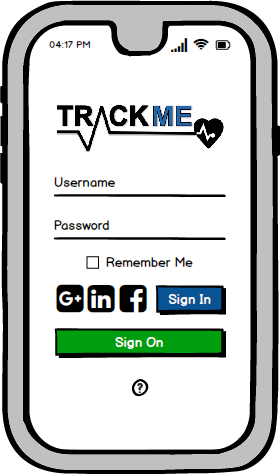
\includegraphics[height=50mm]{images/mockups/Login_Registration.png}
    	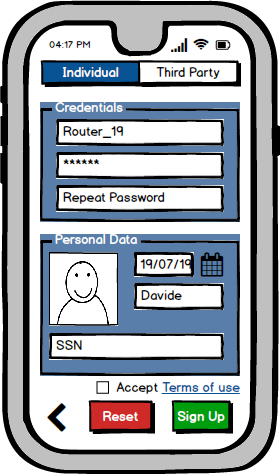
\includegraphics[height=50mm]{images/mockups/RegistrationForm.png}
    	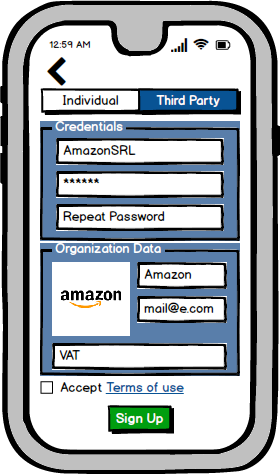
\includegraphics[height=50mm]{images/mockups/ThirdPartyRegistration.png}
        \end{figure}

Once inside the application, the user is redirected to the home page, where he can see the last activities and sign out from \textit{TrackMe}. Swiping left he can access to the profile page which is different whether he is signed in as an Individual or Third-Party. Here the user can access to services provided by \textit{Data4help} and can enable \textit{Automated-SOS} service too. Swiping right instead, the Individual can access to \textit{Track4Run} section.

\begin{figure}[!htpb]
    	\centering
    	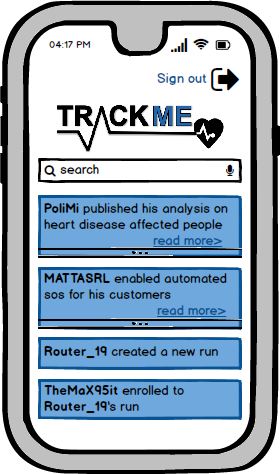
\includegraphics[height=50mm]{images/mockups/HomePage.png}
    	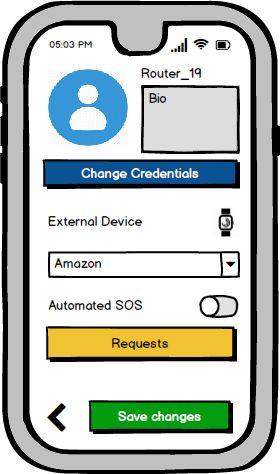
\includegraphics[height=50mm]{images/mockups/IndividualProfile.png}
    	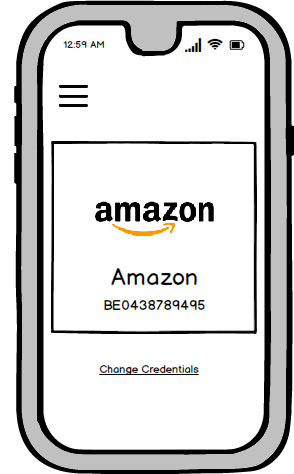
\includegraphics[height=50mm]{images/mockups/ThirdPartyProfile.png}
        \end{figure}

Third-parties can choose either individual or group request and can enable the option to subscribe to new data. The Individuals instead, can handle incoming request by accepting or rejecting them. The Third- Party, form the initial page, can also reach the view data section: here she can see and plot the data of sent requests. Furthermore, swiping left and right, it can move between individual and group data.
\begin{figure}[!htpb]		
		
     	\centering		
     	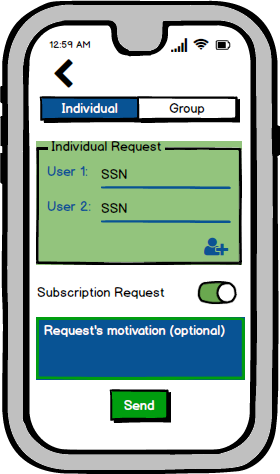
\includegraphics[height=50mm]{images/mockups/Requests.png}		
     	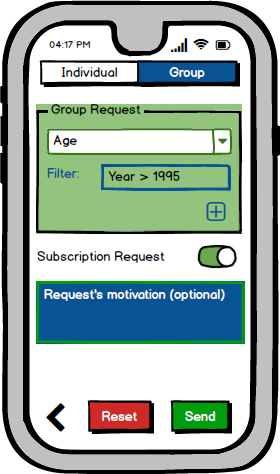
\includegraphics[height=50mm]{images/mockups/GroupRequest.png}		
     	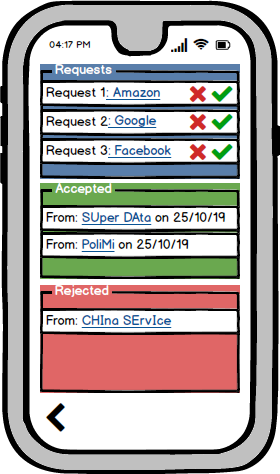
\includegraphics[height=50mm]{images/mockups/ManageRequests.png}		
     	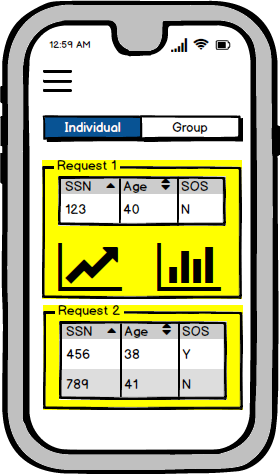
\includegraphics[height=50mm]{images/mockups/ViewData.png}		
     	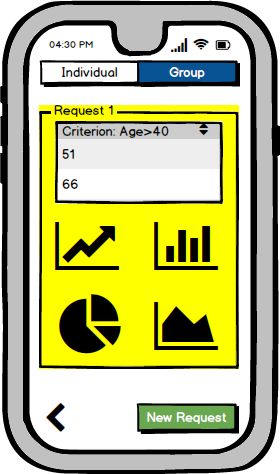
\includegraphics[height=50mm]{images/mockups/ViewData2.png}		
         \end{figure}
        
Once in the \textit{Truck4Run} section, the individual can create, watch, enroll, unroll, start or delete a run.  In the create run page, he can set all the characteristic of the run. Furthermore, he can access to an interactive map to set up the path of the run. In the section watch run there's instead a map with all the position of athletes.

        \begin{figure}[!htpb]
    	\centering
    	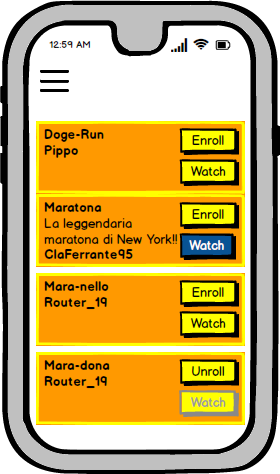
\includegraphics[height=50mm]{images/mockups/RunManager.png}
    	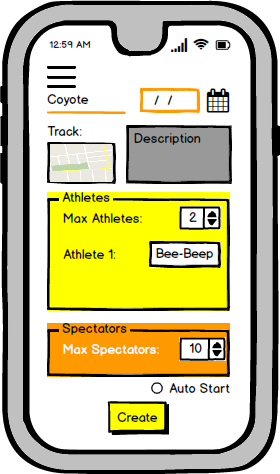
\includegraphics[height=50mm]{images/mockups/RunCreate.png}
    	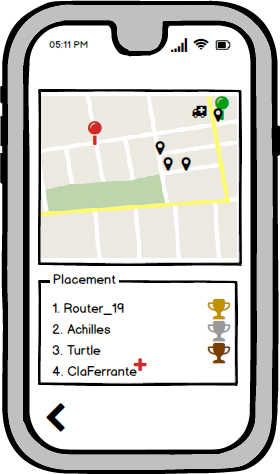
\includegraphics[height=50mm]{images/mockups/ShowMap.png}
    	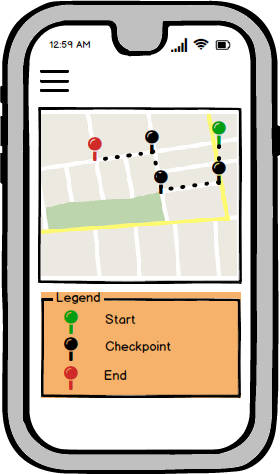
\includegraphics[height=50mm]{images/mockups/DefineTrack.png}
        \end{figure}
     
\subsection{User Experience}
    In this specification we include only mobile users' experience because for web application clients the experience will be the same except for the fact that all \textit{Automated-Sos} and most of \textit{Track4Run} function will be unavailable for web browsers.
    \begin{figure}[!htpb]
    	\centering
    	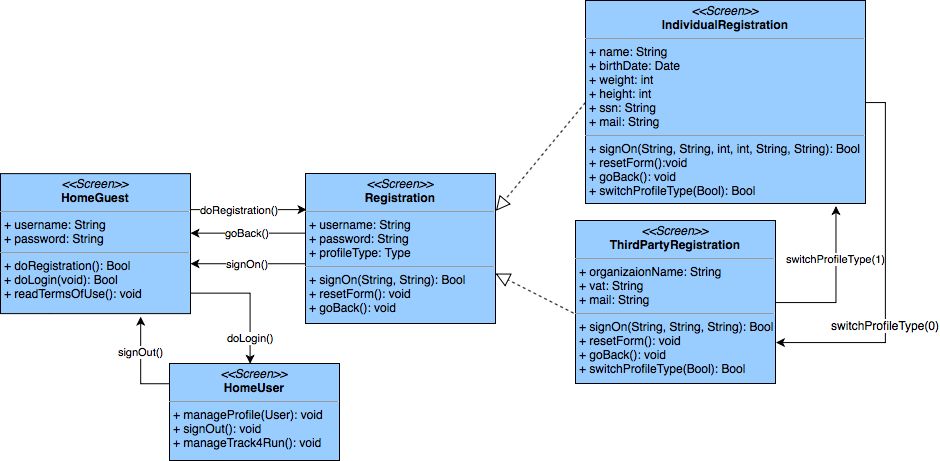
\includegraphics[width=100mm]{images/ux/UX_Guest.png}
    	\caption{Guest eXperience}
    \end{figure}

    \begin{figure}[!htpb]
        \centering
    	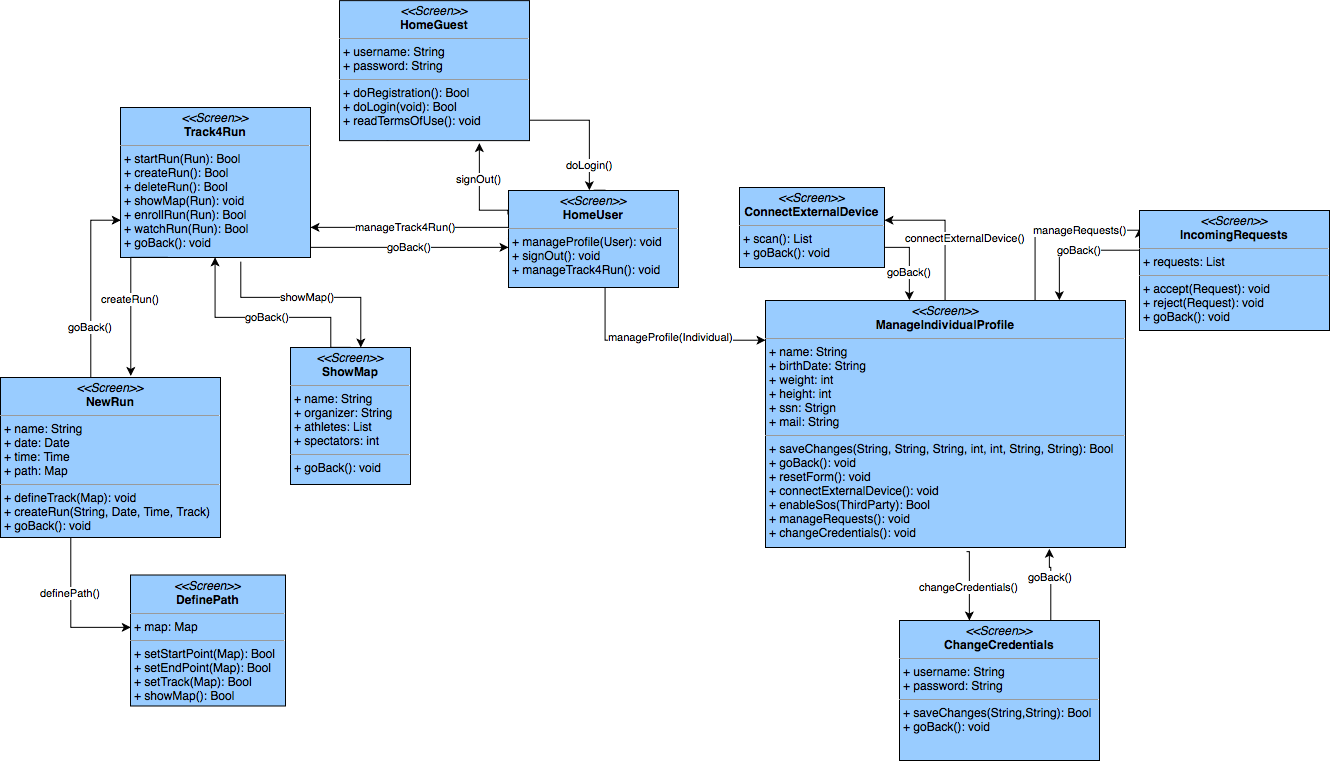
\includegraphics[width=\textwidth]{images/ux/UX_Individual.png}
    	\caption{Individual User eXperience}
    \end{figure}

    \begin{figure}[!htpb]
        \centering
    	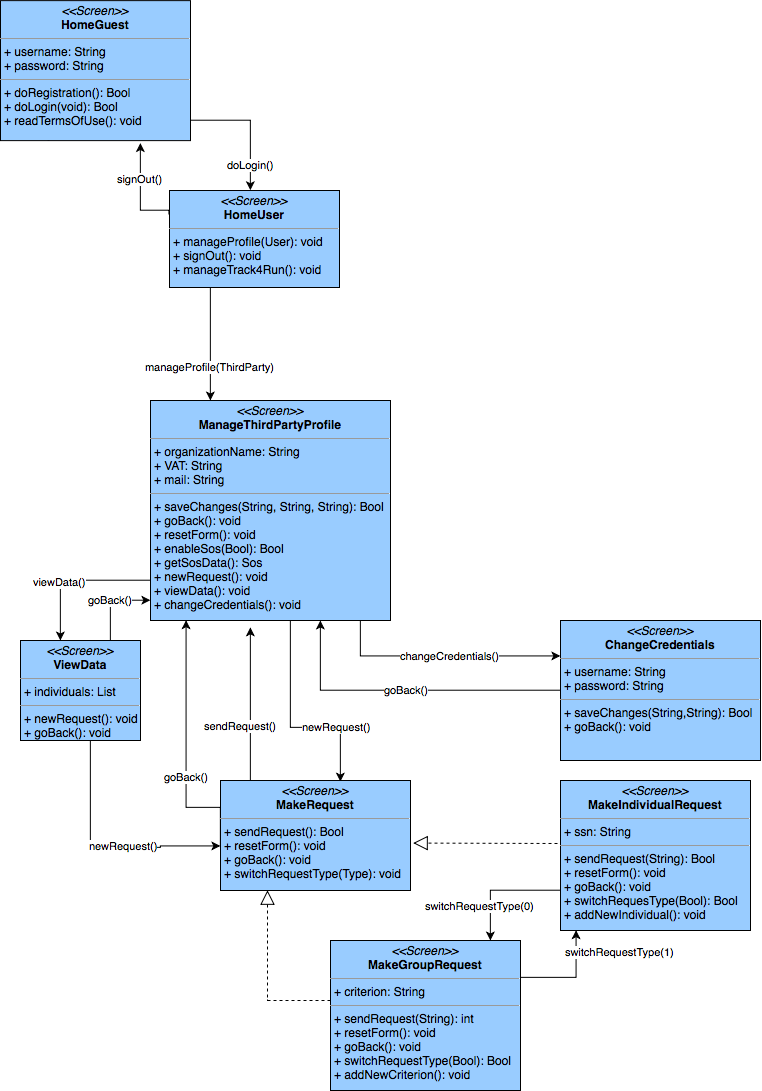
\includegraphics[width=100mm]{images/ux/UX_ThirdParty.png}
    	\caption{ThirdParty User eXperience}
    \end{figure}

\newpage
\section{Requirements Traceability}


\newpage
\section{Implementation, Integration and Test Plan}

\newpage
\section{Effort Spent}
    \begin{itemize}
        \item[-] \textbf{Davide Rutigliano: }
        
        \item[-] \textbf{Davide Matta: }
        
        \item[-] \textbf{Claudio Ferrante: }
    \end{itemize}

\end{document}